% -*- TeX-master: "all_the_notes.tex" -*-

\section{Emission from system}
Before we begin, let us clarify certain assumptions:
\begin{itemize}
\item  \cite{Hoi_2015}  all  the  fields are  reflected  coherent  or
  incoherently.
\item An atom  left to itself in an excited  state \textbf{will never
    decay};
\item Decay only occurs due to  quantum noise. The most trivial case,
  is having two $ Z_0 $ resistors somewhere on the tranmission line:

\begin{figure}[h]
  \centering 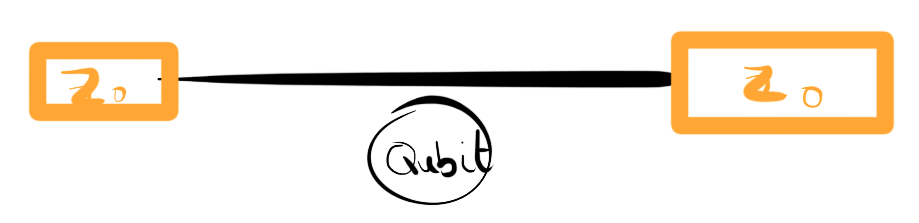
\includegraphics[height=3cm]{noise}
\end{figure}

\noindent

\item  The  quantum  noise  \textbf{\red{which is  the  variation  of
      current squared}} is defined by
  \begin{equation}\label{key}
    S(w) = \red{\iaverage{j^2}} = \frac{1}{Z_0}\hbar\omega
  \end{equation}

  \noindent but only a small part  of it will be affecting relaxation
  of our $ \omega_0 $ qubit.

\begin{figure}[h]
  \centering 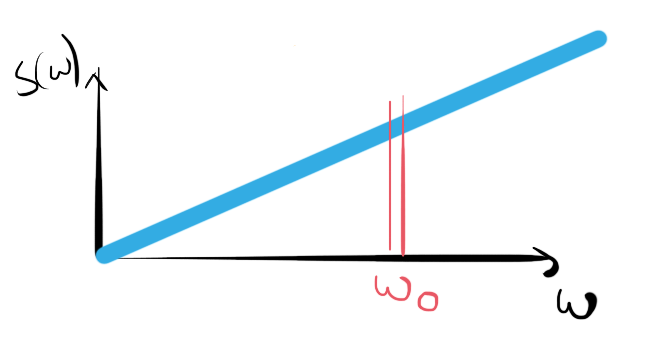
\includegraphics[height=4cm]{noise_spectrum}
\end{figure}

\noindent

\item This mean square current, $ \iaverage{j^2} $ will interact with
  the  flux  being  created  by  the switching  state  of  the  atom,
  $ \vartheta = MI_p\isigmaminus e^{-i\omega t} $, to give an energy

  \begin{equation}\label{key}
    E_\text{interaction}^2 = \iaverage{j^2}\vartheta^2 = \hbar\omega_0\frac{1}{Z_0}\vartheta^2
  \end{equation}

\item  The  frequency associated  with  this  energy (and  hence  the
  transition rate associated with this energy)

  \begin{equation}\label{key}
    \Gamma = \sqrt{\frac{E_\text{interaction}^2}{\hbar^2}} = \cdots (\text{ oleg promised to explain})
  \end{equation}
\end{itemize}

 \subsection{As derived in Oleg's papers \cite{abdumalikov2010}\cite{Astafiev2010}}
 Here it  is written, that relaxation  occur due to quantum  noise in
 the system:
 \begin{equation}\label{key}
   \Gamma_{ij} = \hbar\omega_{ij}\frac{\vartheta_{ij}^2}{\hbar^2Z_0},
 \end{equation}

 \noindent which depends on
 \begin{itemize}
 \item    The   energy    associated   with    the   transition\hfill
   $ \hbar\omega_{ij} $;
 \item    The    dipole     matrix    transition    element    \hfill
   $ \vartheta_{ij} = \bra{i}U\ket{j} \equiv MI_\text{PC}\zeta_{ij}$;
 \item The impedance of the line \hfill $ Z_0 $;
 \end{itemize}

\subsection{Atom emission}
The atom will scatter waves according to
\[
  I_\text{sc}(x,t)                                                  =
  \bigg[i\frac{\hbar\Gamma_{21}}{\phi_{21}}\iaverage{\sigma_{21}}\bigg]e^{ik\iabs{x}-\omega_{21}t},
\]

\noindent  and \iaverage{\sigma_{21}}  is found  from the  stationary
state of  the Master equation  $ \dot{\rho}  = 0 $.  The transmission
coefficient is:

\[
  \begin{aligned}
    t = & \frac{\text{Input current + scattered current}}{\text{Input current}} \ge 1\\
    & = 1 + \big[i\frac{\hbar\Gamma_{21}}{\phi_{21}}\iaverage{\sigma_{21}}\big]\red{e^{ik\iabs{x}-\omega_{21}t}}/\frac{\hbar\Omega_{21}}{\phi_{21}}\quad \red{\text{ignore}}\\
    & = 1 + i\frac{\Gamma_{21}}{\Omega_{21}}\iaverage{\sigma_{21}}
  \end{aligned}
\]

\begin{framed}\noindent
  The relaxation rate is caused by quantum noise in the 1D space:
  \[
    \Gamma_{21}                                                     =
    \hbar\omega_{21}\bigg(\frac{MI_\text{persistent}}{\hbar}\bigg)^2\frac{1}{Z}
  \]

\end{framed}

\subsection{Emission by the atom\label{subsec:Scattering}}
\begin{framed}\noindent
  The input-output theory shows that  the average field emitted by an
  artificial atom to an open transmission line is

\begin{equation}\label{theoEmission}
  \iexpectation{V_{\text{sc}}} =  i\sqrt{\frac{\Gamma_{ij}}{2}}\iexpectation{\sigma_{ji}},
\end{equation}
\end{framed}

\noindent                                                       where
$ \iexpectation{\sigma_{ji}}=\text{Tr}\left\lbrace \iketbra{j}{i}\rho
\right\rbrace   =  \rho_{ij}   $,  and   $  \Gamma_{ij}   $  is   the
\iket{i}\ilra\iket{j} relaxation rate.  The  angular frequency of the
emission is $ \omega_{ij} $.
\begin{itemize}
\item    $   V_{\text{L}}^{+}    $    resonant    input   with    the
  \iket{i}\ilra\iket{j} transition and defined by;
\item  $   V_{\text{L}}^{-}  =   V_{\text{L}}^{+}+V_{\text{sc}}$  the
  transmitted  field, which  is  a combination  of  the incident  and
  emitted  fields\footnote{The   artificial  atom,   whose  dynamics,
    Eq.~\eqref{rwaHamitlonianApprox}, are determined  by the incident
    field, is  treated as a  stand-alone quantum system that  emits a
    field $  V_{\text{sc}} $.  This resultant  field is a sum  of the
    incident, $V_{L}^{+}  $, and emitted, $  V_{\text{sc}} $, fields,
    created by two distinct objects in the quantum system.};
\item $ V_{\text{R}}^{-} = - V_{\text{sc}}$ the reflected field, only
  composed of emission by the artificial atom.
\end{itemize}

The transmission,  $ t  $, and  reflection, $  r $,  coefficients are
defined as

\begin{equation}\label{theoRefTran}
  \begin{aligned}
    t & = \frac{\iexpectation{V_{\text{L}}^{-}}}{\iexpectation{V_{\text{L}}^{+}}} = 1+\frac{i\Gamma_{ij}}{\iexpectation{V_{\text{L}}^{+}}\sqrt{2\Gamma_{ij}}}\rho_{ij};\\
    r                               &                               =
    \frac{\iexpectation{V_{\text{L}}^{-}}}{\iexpectation{V_{\text{L}}^{+}}}
    = 1-t;
  \end{aligned}
\end{equation}

\noindent where $\iexpectation{V} = \frac{1}{T}\int_{0}^{T}V(t)dt$ is
the average voltage  over a normalisation time $ T  $. Since the Rabi
frequency,  $   \Omega  $,  is   related  to  the   drive  amplitude,
$ \iexpectation{V_{\text{L}}^{+}} $,

\begin{equation}
  \Omega_{ij}=\iexpectation{V_{\text{L}}^{+}}\sqrt{2\Gamma_{ij}},
\end{equation}

\noindent Equation~\eqref{theoEmission},  \eqref{theoRefTran}, reduce
to

\begin{equation}\label{theoCoeff}
  \begin{aligned}
    t & = 1 + i\frac{\Gamma_{ij}}{\Omega_{ij}}\rho_{ij};\\
    r & = 1-t.
  \end{aligned}
\end{equation}

\noindent The coefficients of Eq.~\eqref{theoCoeff} apply to coherent
emission, when angular frequencies of  the driving and emitted fields
coincide, $ \omega^{d}_{ij}  \approxeq\omega_{ij} $, and interference
between the onset and emitted waves occur.

  \subsection{Single drive configuration\label{subsec:singleDrive}}
  When  a single  drive couples  two levels  \iket{i}, \iket{j},  the
  non-interacting   third    level   can    be   traced    out   from
  Eq.~\eqref{rawTransformedFinal}.   The  procedure  of  solving  the
  Master  equation,   and  determining~$   \rho  $,  was   done  with
  \texttt{Mathematica}. The $ \rho_{21} $, $ \rho_{31} $ coefficients
  obtained,        for       respective        \iket{1}\ilra\iket{2},
  \iket{1}\ilra\iket{3},     drives,    upon     substitution    into
  Eq.~\eqref{theoCoeff} give

\begin{equation}
  r_{21}=\frac{\Gamma_{21}}{2\gamma_{21}}\frac{1+i\delta\omega_{21}/\gamma_{21}}{1+(\delta\omega_{21}/\gamma_{21})^2+\Omega_{21}^2/\Gamma_{21}\gamma_{21}}; \quad r_{31}=\frac{\Gamma_{31}}{2\gamma_{31}}\frac{1+i\delta\omega_{31}/\gamma_{31}}{1+(\delta\omega_{31}/\gamma_{31})^2+\Omega_{31}^2/\Gamma_{31}\gamma_{31}},
  \label{singleReflectance}
\end{equation}

Figure~\ref{singleDriveReflection}  shows  the   real  components  of
$ r_{ij} $ as function of the  detuning of the driving field from the
atomic                                                    transition,
$ \delta\omega_{ij}  = \delta\omega_{ij}^{d}-\delta\omega_{ij}$.  The
reflectance peak corresponds to the case when the atom relaxes to the
ground state, and  emits a photons that  is coherent~\footnote{Of the
  same frequency.}  with  the incident field, but shifted  by a phase
of   $  \pi   $.\footnote{Signified  by   the   $  i   $  factor   in
  Eq.~\eqref{theoCoeff}.}  Destructive  interference occurs  with the
incident field and the wave is fully reflected.

\begin{figure}[h]
  \centering
  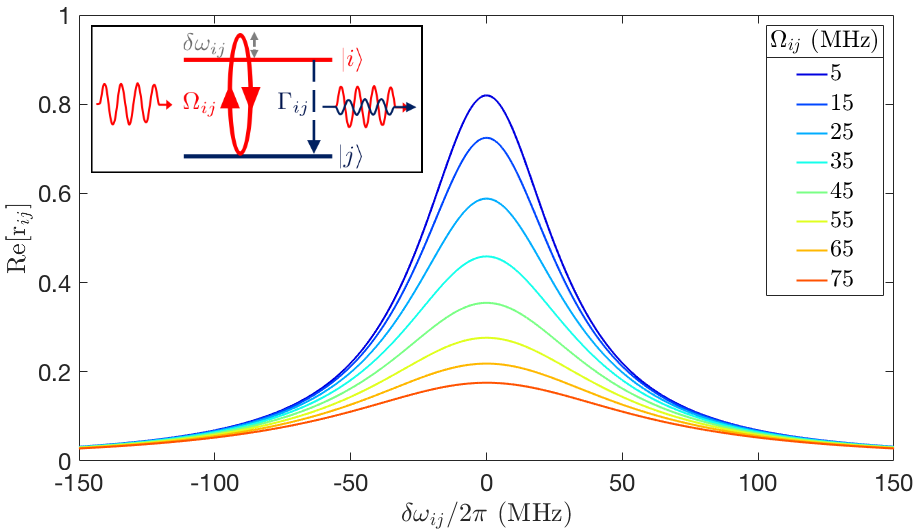
\includegraphics[height=5cm]{transmission_purely_theoretical}
  \caption{\small  \textbf{Simulations of  elastic  scattering of  an
      incident        microwave         in        an        arbitrary
      $  \mathbf{\ket{i}, \ket{j}},  $ system}.   Shown are  the real
    part of  the reflection  coefficient, $ \Re(r_{ij})  $, evaluated
    with               Eq.~\eqref{singleReflectance}              for
    $ \Gamma_{ij}=50,  \Gamma_{\phi,ij}=5 $,  for a range  of driving
    powers, $ \Omega_{ij} $.  When the incident field is on resonance
    with  the   atomic  transition,  $  \delta\omega_{ij}=0   $,  the
    reflectance  curve   exhibits  a  peak,  as   emission  from  the
    artificial  atom   undergo  destructive  interference   with  the
    incident wave.  The  weaker the driving power,  the stronger this
    interference becomes.}
  \label{singleDriveReflection}
\end{figure}

The sharpness of  the central features diminishes  for larger driving
amplitudes, $ \Omega $. As the  number of photons in the transmission
line grows, the photon emitted by  the atom cannot interfere with all
the  ones  propagating  down  the  transmission  line.   This  photon
overload causes  $ t  $ and  $ r  $ to  become insensitive  to atomic
transitions.   To  saturate  the   peak,  one  applies  weak  drives,
$    \Omega_{ij}<<\Gamma_{ij}\gamma_{ij}    $     in    which    case
Eq.~\eqref{singleReflectance}  no  longer   depends  on  the  driving
amplitude

\begin{equation}
  \begin{aligned}
    \Re[r_{21}                                                     ]=
    \frac{\Gamma_{21}}{2\gamma_{21}}\frac{1}{1+(\delta\omega_{21}/\gamma_{21})^2};
    \quad
    \Re[r_{31}]=\frac{\Gamma_{31}}{2\gamma_{31}}\frac{1}{1+(\delta\omega_{31}/\gamma_{31})^2},
  \end{aligned}
  \label{singleLorentzian}
\end{equation}

\noindent   allowing   on   to  determine   the   decoherence   rates
$ \gamma_{ij}, \Gamma_{ij} $ from fittings to observed values.

\begin{framed}\noindent
  The typical Lorentzian has the form

\begin{equation}
  L(d\omega) = A \frac{\gamma}{d\omega^2 + \gamma^2}
\end{equation}

\noindent   which   has  a   \textbf{Full-Width-At-Half-Maximum}   of
$2\gamma$. Rewritting

\begin{equation}
  \frac{\Gamma_{ij}}{2\gamma_{ij}}\frac{1}{1+(\delta\omega_{ij}/\gamma_{ij})^2} \Rightarrow \left[\frac{\Gamma_{ij}}{2}\right] \frac{\gamma}{d\omega_{ij}^2 + \gamma_{ij}^2}
\end{equation}

\noindent we see that

\begin{equation}
  \gamma_{ij} = \frac{\text{Full width at half maximum}}{2}.
\end{equation}

\noindent
\end{framed}

\subsection{Combining the sections above}
Emission from a system is linked to the voltage operator, $ V^{+} $.
\begin{itemize}
\item The voltage operator is defined as:

  \begin{equation}\label{feb22018}
    \hat{V}^{+} = i\frac{\hbar\Gamma_1}{\phi}\sigma^{-},
  \end{equation}

  \noindent the `-' coming from the  fact that the atom must relax in
  order for voltage to be  produced. The average produced field would
  be

  \[
    \iaverage{\hat{V}^{+}}                                          =
    i\frac{\hbar\Gamma_1}{\phi}\iaverage{\sigma^{-}},
  \]

\item  Now,  the   power  resulting  from  this   voltage,  which  is
  effectively noise as the atom relaxes spontaneously, can be found:

  \begin{equation}\label{feb22018:1}
    \begin{aligned}
      \iaverage{V^2(\omega)} = & \frac{1}{2\pi}\int_{-\infty}^{\infty}\iaverage{\hat{V}^{-}(0)\hat{V}^{+}(\tau)}e^{i\omega \tau}d\tau\\
      =                                                             &
      \frac{\hbar^2\Gamma_1^{2}}{\phi^2}\frac{1}{2\pi}\int_{-\infty}^{\infty}\iaverage{\sigma_{+}(0)\sigma_{-}(\tau)}e^{i\omega
        \tau}d\tau
    \end{aligned}
  \end{equation}

\item \red{Using  a trick in Olegs  book, one can find  that the term
    $  \iaverage{\sigma_{+}(0)\sigma_{-}(\tau)} $  can be  decomposed
    as:
    \begin{itemize}
    \item \textbf{Total sum is} \[ \frac{1+{\isigmaz}}{2}. \]
    \item \textbf{The coherent part is}
      \[ \iaverage{\sigma_{+}}\iaverage{\sigma_{-}}. \]
    \item  \textbf{Therefore   the  incoherent   part  must   be  the
        difference between the two}:
      \[                   \frac{1+{\isigmaz}}{2}                   -
        \iaverage{\sigma_{+}}\iaverage{\sigma_{-}}. \]
    \end{itemize}
  }

\item Finding the  total emitted power, by integrating  over the full
  frequency  range  \red{and  assuming   that  we  are  dealing  with
    stationary  states  (ss)  that  would form  in  the  system  when
    averaging:}

  \begin{equation}\label{feb220183}
    \begin{aligned}
      \text{Power}_\text{total} &= \frac{1}{Z}\int   \iaverage{V^2(\omega)}  d\omega\\
      & = \frac{1}{Z}\int \frac{\hbar^2\Gamma_1^{2}}{\phi^2}\frac{1}{2\pi}\int_{-\infty}^{\infty} \frac{1+{\isigmaz}_{ss}}{2} e^{i\omega \tau}d\tau   d\omega\\
      & = \frac{\hbar^2\Gamma_1^2}{Z\phi^2} \frac{1+{\isigmaz}_{ss}}{2} \int\frac{1}{2\pi}\int e^{i\omega\tau}d\tau d\omega\\
      & \text{Using the fact that the integral over the delta function is just 0 and } \Gamma_1 = \frac{\hbar\omega\phi^2Z}{\hbar^2}\\
      & = \hbar\omega\Gamma_1 \frac{1+{\isigmaz}_{ss}}{2}
    \end{aligned}
  \end{equation}

  \noindent Now, because we are driving continously, decoherence will
  result in  our rotation of the  state from \iket{0} to  \iket{1} to
  form an intermediate value when $ \isigmaz = 0 $ and so the maximum
  emitted power from the atom will be:

  \begin{framed}\noindent
    \begin{equation}\label{key} \text{Power}_\text{total} =
      \frac{\hbar\omega\Gamma_1}{2}
    \end{equation}
  \end{framed}


\item  Now,  redoing the  same,  but  only considering  the  coherent
  contribution i.e.   instead of $ \frac{1+{\isigmaz}_{ss}}{2}  $ use
  $ \iaverage{\sigma_{+}}\iaverage{\sigma_{-}} $ we round up at:

  \begin{equation}\label{maximalCoherentEmission}
    \begin{aligned}
      \text{Power}_\text{coherent} &= \hbar\omega\Gamma_1 \iaverage{\sigma_{+}}_{ss} \iaverage{\sigma_{-}}_{ss} = \text{ upon subbing in the obtained expectation values }\\
      &                                                             =
      \hbar\omega\Gamma_1\bigg(\frac{2\Gamma_1\Omega}{2\Gamma_1^2+\Omega^2}\bigg)\\&\Rightarrow
      \text{max value } = \frac{\hbar\omega\Gamma_1}{8}
    \end{aligned}
  \end{equation}

  \begin{itemize}
  \item  \red{You can  measure  this  power with  the  SPA i.e.   you
      measure 1/8 of a single photon power;}
  \item Then, you can  tune your VNA power to match  this $ 8\times $
    coherent signal power, and be supplying exactly one photon to the
    system.  Then  there will be no  leakages, as the photon  will be
    absorbed by the system, with no leftover for leaking;
  \end{itemize}
\item The total number of photons in the system can be found from
  \begin{equation}\label{key}
    N = \frac{\Omega}{\Gamma_1}
  \end{equation}
\end{itemize}

\newpage

\subsection{Coherent and incoherent emission}
\begin{enumerate}
\item \textbf{Coherent field}, means a  fixed phase relation with the
  two input  fields.  For example,  supplying $ e^{i\omega_1t}  $ and
  $  e^{i\omega_2t}  \ira  e^{i(\omega_1+\omega_2)t  +  \phi}$  where
  $  \phi  $ is  a  fixed  value.   This allow  further  entanglement
  procedures;
\item \textbf{Emission by qubit} can be characterised as coherent and
  incoherent emission.   One needs  to work  with \iaverage{\sigma_i}
  values and look at the corresponding bloch sphere.

  \begin{figure}[h]
    \centering 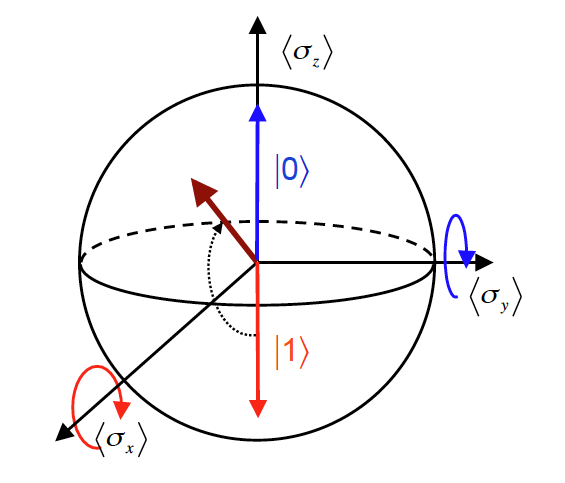
\includegraphics[height=7cm]{sphere}
  \end{figure}

  Recalling that

  \red{{\large  \begin{equation}\label{expectationPauli} \rho_{00}  =
        \frac{\iaverage{\sigma_z}+1}{2};\quad
        \rho_{01}=\frac{\iaverage{\sigma_x}-i\iaverage{\sigma_y}}{2}
        =
        \iaverage{\sigma_{+}};\quad\rho_{10}=\frac{\iaverage{\sigma_x}+i\iaverage{\sigma_y}}{2}
        = \iaverage{\sigma_{-}};
      \end{equation}
      \begin{equation}\label{expectationPauli2}
        \iaverage{\sigma_x}=\rho_{01}+\rho_{10};\quad\iaverage{\sigma_y} = i\rho_{01}-i\rho_{10};\quad\iaverage{\sigma_z}=\rho_{00}-\rho_{11}
      \end{equation}}}

  \noindent The more a state is on the equator, the more coherence it
  has since a superposition is formed.  Recall that, so that when the
  ``arrrow'' projects fully onto the  equator, it means that the atom
  is         in        a         superposed        state         e.g.
  $              \frac{\iket{0}+\iket{1}}{\sqrt{2}}              \ira
  \imatrixfour{1/2}{1/2}{1/2}{1/2} \ira \isigma_z = 0, \isigma_x = 1$
  (or some other rotation around y).

  \begin{center}
    \textbf{Coherent emissions $ \propto \isigmax$\newline Incoherent
      $ \propto\isigmaz $. \large}
  \end{center}
  \red{Both  emissions  will occur  at  the  frequency of  the  qubit
    $ \omega_0 $  (i.e.  energy level separation),  but emission from
    \isigmax will  be sharp, while incoherent  emission from \isigmaz
    will be broad as shown below}

\begin{figure}[h]
  \centering 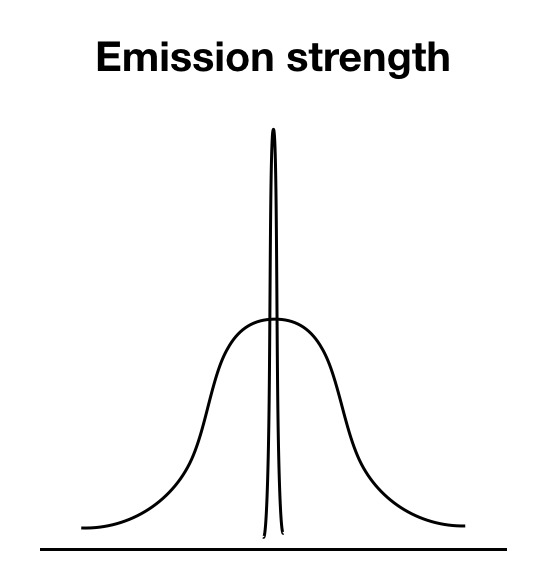
\includegraphics[height=5cm]{emission}
\end{figure}

\noindent
\item Now draw the parrallels between:

  \begin{itemize}
  \item The field in a resonator \hfill a and \iadagger;
  \item                     Qubit\hfill                    excitation
    $  \sigma_{+}  =   \iketbra{1}{0}  =  \imatrixfour{0}{0}{1}{0}  =
    (\sigma_x-i\sigma_y)/2$               and              relaxation
    $  \sigma_{-}  =   \iketbra{0}{1}  =  \imatrixfour{0}{1}{0}{0}  =
    (\sigma_x+i\sigma_y)/2$

  \end{itemize}
  in the following way

  \begin{center}
    \begin{tabular}{|c|c|c|}
      \hline
      \textbf{Coherent field} & $ \big(a + \iadagger\big) $ & $ \isigmax $ \\
      \hline
      \textbf{Photon number} & $ a iadagger $& \isigmaz \\
      \hline
    \end{tabular}
  \end{center}

\end{enumerate}
\newpage
